\documentclass[12pt,onecolumn,a4paper]{article}
\usepackage{float}
\usepackage{epsfig,graphicx,subfigure,amsthm,amsmath}
\usepackage{color,xcolor}
\usepackage{xepersian}
\usepackage{graphicx}
\usepackage{placeins}

\settextfont[Scale=1.2]{BZAR.TTF}
\setlatintextfont[Scale=1]{Times New Roman}


\begin{document}
\title{\lr{ENVISION OF PRODUCT} \\ پلتفرم اینترنتی فروش پوشاک}
\author{امیرمحمد فتاحی\\95102073 \and آرزو کاظمی دولت آبادی \\9194222 \and امیرحسین ایمانی\\96104087}
\date{\today}
\maketitle

\newpage
\tableofcontents
\newpage
\listoffigures
\newpage


\section{فاز اول: محدودیت محصول}
\subsection{تطبیق پذیری :}

سایت ما باید بتواند با شرایط مختلف تطبیق پذیرد و سازگار شود . برای مثال در صورت عدم موجودی سایت بلافاصله آپدیت شود و عدم موجودی را نمایش دهد . درصورت عدم وجود این موضوع مشتریان نارضایتی از محصول ما خواهند داشت . همچنین سایت باید با تکنولوژی های جدیدی که می آید به روز شود تا سهولت استفاده برای کاربران ایجاد کند .
\subsection{قابلیت اطمینان }
کاربران از ما انتظار دارند که 24 ساعته به آن ها سرویس بدهیم و در سرویس دهیمان وقفه به وجود نیاید . در واقع این ویژگی به انتظار کاربران به استفاده مداوم از پلتفرم ما باز میگردد . کاربران از ما انتظار دارند زمان در دسترس نبودن سایت به دلیل مسائل مختلف و فاصله ی بین این اتفاقات به حداقل خود برسد .

\subsection{مقیاس پذیری }
مقیاس پذیری باید در تکنولوژی ما باشد و بتوانیم با رشد غیر قابل پیش بینی تقاضا به هنگام شویم و غافلگیر نشویم . باید با استفاده از تجهیزات و ساختار ها و زیر بناهای قوی این مقیاس پذیری را در سایت خود ایجاد کنیم .

\subsection{امنیت}
همه ی فرآیند های اینترنتی امروزه به سطوح مشخصی از امنیت احتیاج دارند . یک نوع از امنیت به معنای حفاظت از مشتری می باشد و دیگری به حفاظت از شرکت می باشد . مهندسان سایت ما باید با وقت گذاری تاثیر عدم امنیت در سازمان را متوجه شوند و در صدد حفاظت از آن برآیند .  عمل امنیت باید در دو جبهه صورت گیرد : 1. حفاظت از اینترنت در برابر اسکمر ها 2. حفاظت از شرکت در مقابل دزدان

\subsection{قابلیت استفاده}
در دنیای امروزه قدرت در دست مشتریان قرار دارد . قابلیت استفاده یک محدودیت کالا است که به قدرت مشتری در استفاده از سایت ما باز میگردد . این ویژگی باید شامل
1.	حداکثر زمان بهینه ی پاسخگویی
2.	دسترسی 24 ساعته 7 روز در هفته
3.	قابلیت شخصی سازی نمایش سایت
4.	قابلیت فیلتر کردن اطلاعات
5.	قابلیت انتخاب محصولات
مهم ترین نکته ، در این نکته این است که چند کلیک طول میکشد تا به اطلاعات مورد نظر برسد و یا چرخه ی خود را تکمیل کند .

\subsection{قابلیت نگهداری}
هر چند ماه یکبار قابلیت های جدید به نرم افزار اضافه شود . یک نیازمندی نگهداری باید توسط صاحب سایت مشخص شود و طبق آن پیش رفت .


\section{نیازمندی های کارکردی}
\subsection{ثبت نام مشتری :}
1. ورود به سامانه\\
2. ثبت شماره همراه یا ایمیل \\
3. تکمیل مشخصات\\
4. دریافت پیامک تایید \\
5. تکمیل ثبت نام\\
\\
\\
\subsection{
ثبت نام صاحب فروشگاه  :
}
1. مراجعه حضوری\\
2. تکمیل مشخصات فروشگاه اعم از ساعت کاری و آدرس\\
3. عقد قرارداد با شرکت\\
4. ثبت در سامانه\\
5. دسترسی به سایت \\
6. امکان حذف و ویرایش و اضافه کردن محصولات به همراه مشخصاتشان\\
\\
\\

\subsection{
ثبت نام پیک موتوری  :
}
1. مراجعه حضوری\\
2. ثبت مشخصات خود\\
3. ثبت مشخصات وسیله نقلیه\\
4. ثبت در سامانه\\

\subsection{
ثبت درخواست توسط مشتری :
}
1.	ورود به سامانه\\
2.	دریافت لیست فروشگاه های نزدیک\\
3.	دریافت قیمت پیک\\
4.	انتخاب فروشگاه مد نظر\\
5.	مشاهده کالاهای موجود\\
6.	ایجاد سبد خرید شامل محصولات و تعداد آن ها\\
7.	انتقال به درگاه بانک\\
8.	پرداخت هزینه در سامانه از طریق درگاه بانک\\
9.	مشاهده موفقیت آمیز بودن تراکنش\\
10.	درصورت عدم موفیت تراکنش به گام شماره 7 باز میگردد \\
11.	دریافت محصول\\
12.	ارسال نظر و پیشنهاد به فروشگاه\\
13.	ارسال نظر و فروشگاه به پیک موتوری\\

\subsection{
ثبت درخواست ها توسط پیک :
}
1. تامین تلفن همراه به جهت ردیابی\\
2. قبول سفارش\\
3. دریافت اطلاعات خرید اعم از اطلاعات فروشگاه ، آدرس مقصد و لیست خرید \\
4. تحویل سفارش به مشتری\\

\subsection{
ثبت درخواست مرجوعی توسط مشتری :
}
1.	تماس با تیم پشتیبانی\\
2.	تحویل کالا به پیک\\

\subsection{
ثبت درخواست توسط صاحب فروشگاه :
}
1.	دریافت لیست خرید\\
2.	آماده سازی سبد خرید\\
3.	تحویل سفارش به پیک\\

\subsection{
ثبت درخواست توسط سیستم :
}
1.	نمایش لیست فروشگاه های نزدیک به مشتری و هزینه ارسال پیک\\
2.	بررسی لیست کالا های سفارش مشتری\\
3.	دریافت هزینه توسط درگاه بانک\\
4.	بررسی پیک های موتوری آنلاین\\
5.	انتخاب پیک موتوری\\
6.	نمایش اطلاعات خرید اعم از اطلاعات فروشگاه ، آدرس مقصد و لیست خرید\\
7.	درصورت رد درخواست توسط پیک مجددا جستجو انجام میگیرد\\
8.	دریافت و ذخیره امتیازات و نظرات\\
9.	نمایش امتیازات و نظرات\\

\newpage
\section{برد چشم انداز محصول\cite{3}(\lr{Product Vision Board})}
\begin{figure}[!h]
\centering{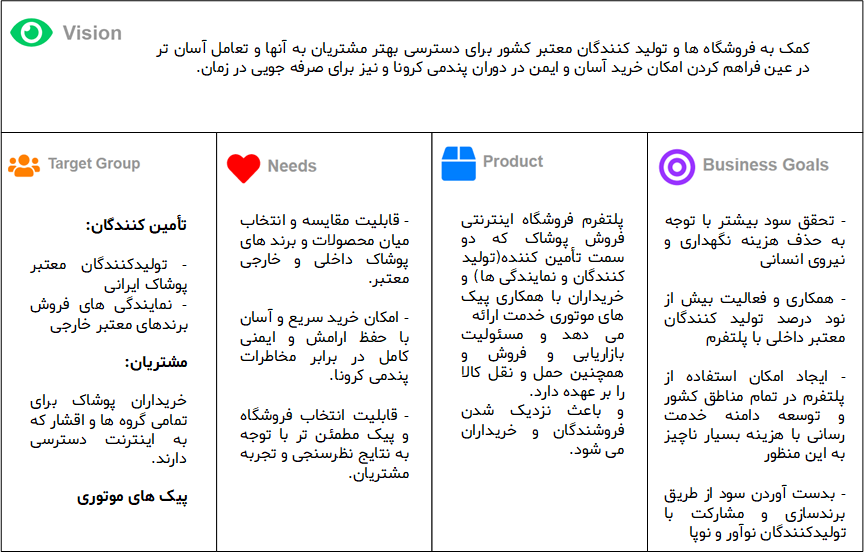
\includegraphics[width=14cm]{product_vision_board}}
\caption{\lr{product vision board}}\label{figpvb}
\end{figure}



\newpage

\section{داستان کاربری: }


\subsection{مقدمه}
داستان کاربر ابزاری است که در توسعه نرم افزار (چابک) به کار برده میشود تا خصوصیات یک نرم افزار را از دیدگاه یک کاربر نظاره گر باشد. داستان کاربر به شما میگوید که مخاطبان شما چه کسانی هستند، چه چیزی می خواهند و چرا؟
همان طور که بیان شد داستان کاربری یکی از راهکارهای دیدگاه چابک است. به این صورت که تمرکز از روی نیازها برداشته میشود و به تجربه کاربران و نظرات انها میپردازد.\\
\begin{figure}[h]

\includegraphics[scale=0.5]{cj}
\end{figure}

\subsection{ کاربران }
 1. مشتری 2. صاحب فروشگاه 3. پیک موتوری

\subsubsection{ مشتری }

به عنوان یک مشتری میخواهم پس سفارش خیلی سریع محصول به دستم برسد و در نزدیکی زمان تحویل  پیامکی جهت اینکه مطلع باشم که محصول به من خواهد رسید داشته باشم تا بتوانم حضور پیدا کنم.\\
\\
	

به عنوان یک مشتری میخواهم در سایت امکان فیلتر گذاری باشد (دخترونه و پسرونه یا از نظر قیمت یا سن) تا سریع تر بتوانم محصول خود را پیدا و انتخاب کنم.\\
\\


من به عنوان یک مشتری می‌خواهم که وقتی کالایی را در سایت برررسی میکنم دیتا ها   در لحظه باشد یعنی اگر کالا موجود نیست اطلاع رسانی شود تا محصول نا موجود را به اشتباه انتخاب نکنیم .\\
\\


به عنوان یک مشتری میخواهم نظرسنجی هاخیلی بررسی شود تا در مراحل بعدی مشکلی پیش نیایید و برطرف شود.\\
\\


به عنوان یک مشتری میخواهم فرایند خرید راحت و واضح باشد تا بتوانم با خیال اسوده خرید را انجام دهم.\\


به عنوان یک مشتری میخواهم اطلاعات جامع و کاملی از محصول اعم از جنس پارچه تا دچار مشکلاتی مانند پس فرستادن و نپذیرفتن از جانب شرکت نشود.\\
\\


به عنوان یک مشتری میخواهم کاربران سایت ما را راهنمایی کنند تا به مشکل برنخوریم.\\
\\

... چند هفته قبل اطلاع رسانی شود تا بتوانیم برنامه ریزی کنیم.\\
\\


به عنوان مشتری میخواهم در صورت داشتن مشکلی در کالا فروشگاه ان کالا را پس بگیرد تا حس رضایت و اعتماد بیشتر شود.\\
\\


به عنوان مشتری میخواهم در صورت رسیدن به یک عددی در خرید تخفیف ویژه به مشتریان بدهند تا وفاداری و حس خوب بیشتر شود به این سایت و....\\
\\

 تماس تلفنی و ... انجام شود تا بتوانم مشتری دائم شوم و فرایندها را یاد بگیرم و بیشتر خرید کنم.\\
\\

 برخورد مناسبی داشته باشند تا حس اعتماد بدست اورم و خرید بیشتری انجام دهم.\\
\\




\subsubsection{ صاحب فروشگاه  }

	  به عنوان یک صاحب فروشگاه میخواهم بعد از ارسال کالا یک نظر سنجی گذاشته شود تا سطح رضایت افراد را متوجه شویم چه از نظر به موقع بودن و چه از نظر کالای انتخابی\\
	  \\

 چه سمت و سویی است و بیشتر در چه رنج سنی و چه جنسیتی دارند.\\
\\


به عنوان یک صاحب فروشگاه گزارش می‌خواهم پیک موتوری سریع حاضر شوند و خیلی سری
ع مرسوله را به دست مشتری برسانند تا مشتریان به ما اعتماد کنند.\\
\\


 شود تا هم مشکلاتشان برطرف شود هم افراد دیگر هم با خواندن سوالات در صورت مشکل بتوانند انرا برطرف کنند.\\
\\


به عنوان یک صاحب فروشگاه گزارش می‌خواهم اطلاعات سریع اپدیت شود تا مشتریان به مشکل برنخورند و از خدمات راضی باشند.\\
\\


به عنوان یک صاحب فروشگاه گزارش می‌خواهم از نظر فنی سایت عالی باشد(سرعت و طراحی و...) تا مشتری لذت ببرد و حس رضایت داشته باشد و وفادار بماند.\\
\\


به عنوان یک صاحب فروشگاه می‌خواهم اطلاعات کالا را به خوبی بخوانند تا در صورت دریافت کالا مشکلی از لحاظ مثلا جنس پارچه و .... نداشته باشند.\\
\\


به عنوان یک صاحب فروشگاه می‌خواهم پول محصول را در کوتاه ترین زمان دریافت کنم تا بتوانم خریدهای اتی را انجام دهم.\\
\\










\subsubsection{پیک موتوری}

  من به عنوان یک پیک موتوری انتظار دارم که مشتریان ادرس را به صورت کامل و جامع ارسال کنند تا در جست و جوی مسیر مشکلی پیش نیاید.\\
  \\


من به عنوان یک پیک موتوری انتظار دارم شرکت تسهیلاتی را برای قائل شوند.\\
\\


به عنوان یک پیک موتوری می‌خواهم که بیمه شوم تا در صورت هر گونه اتفاق و خطری پیگیری شود.\\
\\


به عنوان یک پیک موتوری می‌خواهم رفتار خوبی از مشتریان داشته باشم تا انگیزه بگیرم برای ادامه کار.\\
\\


به عنوان یک پیک موتوری میخواهم در صورت راضی بودن امتیاز و نظر بدهند تا در صورت به دست اوردن امتیاز بالا پاداش دهند.\\
\\



\section{فاز دوم :نمودار توالی فرآیند فروش}
\subsection{\lr{Actur} }

1. مشتری
2. پیک

طبق دلایل یاد شده فروشگاه در این بخش تعریف نشده.
\subsection{\lr{Subject} }
1. سایت
2. فروشگاه
3. بانک

صفحه پرداخت و دیگر جزئییات بدون در نظر گرفتن صدا زدن \lr{Api} تصویر شده و به دلیل ساده سازی فرآیند سایت شامل تمامی بخش ها و دیتابیس و ... فرض شده

\subsection{فرضیات }
برای این فرآیند فرض قابل توجهی غیر از موارد تعریف شده در پروژه دیده نشده چون موارد یاد شده به نسبت بخش های دیگر کامل شرح داده شده.

\newpage
\begin{figure}[!h]
\centering{
\includegraphics[width=14cm]{Sequence_Diagram_Buy}}
\caption{نمودار توالی فرآیند فروش}\label{sellpng}
\end{figure}


\section{نمودار توالی فرآیند فروش}
\subsection{\lr{Actur} }

1. مشتری
2. پیک

طبق دلایل یاد شده فروشگاه در این بخش تعریف نشده.
\subsection{\lr{Subject} }
1. سایت
2. فروشگاه
3. بانک

صفحه پرداخت و دیگر جزئییات بدون در نظر گرفتن صدا زدن \lr{Api} تصویر شده و به دلیل ساده سازی فرآیند سایت شامل تمامی بخش ها و دیتابیس و ... فرض شده

\subsection{فرضیات }
برای این فرآیند فرض قابل توجهی غیر از موارد تعریف شده در پروژه دیده نشده چون موارد یاد شده به نسبت بخش های دیگر کامل شرح داده شده.

\newpage
\begin{figure}[!h]
\centering{
\includegraphics[width=14cm]{Sequence_Diagram_Buy}}
\caption{نمودار توالی فرآیند فروش}\label{sel1lpng}
\end{figure}


\section{نمودار توالی مرجوع کردن کالا}
\subsection{\lr{Actor} }
1. مشتری
2. پیک
به دلیل اینکه فروشگاه به عنوان یک مجموعه دیده شده که ممکن است بخش های مختلف داشته باشد آنرا بعنوان اکتور در نظر نگرفتیم.

\subsection{\lr{Subject} }
1. سایت
2. واحد پشتیبانی شرکت
3. فروشگاه
\subsection{فرضیات }

به دلیل ساده سازی دیگر در این فرآیند بخشهای مختلف سایت و جزئییات فنی همه به عنوان مجموعه ای به نام سایت در نظر گرفته شده.
از طرفی فروشگاه پس از دریافت کالای مرجوعی وجه را به خریدار پس می دهد.

\newpage
\section{ \lr{Use Case}    }
\begin{figure}[!h]
\centering{\includegraphics[width=14cm]{usec1}}
\end{figure}

\newpage

\begin{figure}[!h]
\centering{\includegraphics[width=14cm]{usec2}}
\end{figure}

\newpage
1.فرض بر این است که ما به جای سامانه اکتور هایی را مشخص کنیم تا مسئول دریافت اطلاعات یا شروع کننده یوز کیس باشند مانند   مسئول سایت.\\
2.در هنگام دریافت محصول یوز کیس تحویل سفارش در فرایند ارسال انجام شده است پس فقط در فرایند دریافت سفارش یوز کیس ارسال نظر میماند.\\
3.همه این \lr{Use Case} در یک سیستم سفارش انلاین موجود هستند ولی چندتا از این یوز کیس ها یک فرایند را تشکیل میدهند به همین علت یک \lr{Use Case} کلی برای فرایند در نظر میگیریم و این \lr{Use Case}ها یه صورت \lr{Include}به انها متصل میشوند.\\ زیرا باید تمامی \lr{Use Case} ها انجام شود تا ان فرایند صورت گیرد.\\
4.قسمت های شرطی چون احتمالی هستند و ممکن است رخ دهند یا رخ ندهند به صورت \lr{ extend}درنظر میگیریم.


\begin{figure}[!h]
\centering{\includegraphics[width=14cm]{usecase}}
\caption{  نمودار یوزکیس }\label{usecase}
\end{figure}

\newpage
\section{ \lr{Activity Diagrams }    }


\begin{figure}[!h]
\afterpage{\FloatBarrier}
\centering{\includegraphics[width=14cm]{orderfulfilment}}
\caption{   نمودار اکتیویتی سفارش }\label{ordact}
\end{figure}



\begin{figure}[!h]
\centering{\includegraphics[width=14cm]{registeract}}
\caption{   نمودار اکتیویتی ثبت نام }\label{regact}
\end{figure}


\begin{figure}[!h]
\centering{\includegraphics[width=14cm]{reverseorder}}
\caption{   نمودار اکتیویتی بازگشت کالا }\label{revact}
\end{figure}

\section{فاز سه: نمودار مدل\lr{BPMN} فرآیند خرید}
\subsection{توضیحات مدل }

در نمودار مدل ایجاد شده پیک را به دلیل اینکه از ابتدا تا انتها با پلتفرم درگیر است بعنوان \lr{lane}  در کنار بخش فروش سایت در یک \lr{pool} به نام وب‌سایت فروش در نظر گرفته شده و دیگر بخش ها همان‌‌طور که در نمودار مشخص است شامل: بانک، مشتری و فروشگاه بعنوان \lr{pool} است.
فرآیند پرداخت نیز در توالی مربوط به مشتری به دلیل مجزا بودن از کل فرآیند و به نوعی فرا بخشی بودن در یک \lr{Sub- process} شده.
به دلیل چالش‌ها و نقص‌ها نرم افزار \lr{Bizagi} که نه تنها امکان انتقال از درون یک \lr{Sub- process} وجود ندارد بلکه اصلاح و ایجاد تغییر در ان نیز به طور کامل امکان‌پذیر نبوده و بعضی بخش ها در تصویر نهایی نمودار ادیت شده.
توالی اطلاع سایت فروش و فروشگاه از ارسال سفارش منطقا اینگونه  فرض شده و فروشگاه تنها پس از دریافت رسید پرداخت محصول را تحویل پیک می‌دهد و به نوعی پیش‌نیازی تبدیل شده.
 برای اجتناب از رسم ارتباطات غیر ضروری میان مشتری و سایت فروش فرض شده که تکمیل کردن مراحل خرید اقدامی از سوی مشتری بوده و به دلیل عدم اطلاع دقیق از کنش و واکنش های سایت تنها در آخرین مرحله پس از پرداخت پیغامی به عنوان رسید و پرداخت و سفارش به وب‌سایت فروش انتقال داده می‌شود.
در آخر باید این نکته را متذکر شویم که این تنها روش مدلسازی این فرآیند نیست و می‌توان و با تغییر فرضیات و جیدمان \lr{Pool , lane}های متفاوت به نحوه دیگری نمودار را رسم کرد اما مهم وجود تمامی فعالیت ها با رعایت توالی آنهاست که در مدل رسم شده به این موضوعات توجه شده.


\subsection{پیشنهاد }
بنده بعد از این تجربه دیگر هرگز از نرم‌افزار \lr{Bizagi} به دلیل نقص‌های زیاد و جدی آن استفاده نخواهم کرد به همین دلیل بعنوان یک پیشنهاد لطفا در ترم‌های آینده نرم‌افزار دیگری جایگزین نمایید.



\newpage
\begin{figure}[!h]
\centering{\includegraphics[width=14cm]{Sell_Bpmn_Diagram}}
\caption{نمودار مدل\lr{BPMN} فرآیند خرید}\label{sellbpmnpng}
\end{figure}

\newpage

\section{نمودار بیزاجی بازگشت کالا}
\begin{figure}[!h]
\centering{\includegraphics[width=14cm]{reverseb}}
\caption{   نمودار بیزاجی بازگشت کالا }\label{revb}
\end{figure}

\section{نمودار بیزاجی  ثبت نام متقاضی }
\subsection{انواع تسک ها}

\lr{User task:} منظور زمانی است که کاربر مدنظر با یک سیستم اقدامات (مانند ثبت نام کاربر که با سیستم، سامانه است) را انجام میدهد.\\
\lr{Manual task:} منظور زمانی است که کاربر مد نظر با یک انسان اقدامات را انجام میدهد(مثلا وقتی صاحب فروشگاه به صورت حضوری با شرکت قرارداد میبندد و فروشگاه با سیستم کاری نمیکند)\\
\lr{end task:} زمانی است که یک اقدام ماهیت ارسالی دارد.\\
\lr{Receive task:} زمانی است که یک اقدام ماهیت دریافتی دارد (مانند دریافت پیامک)\\

\subsection{ فرایند ثبت نام متقاضی: }

در این بخش متقاضی همان کاربر ما است که صرفا ثبت نام میکند و خریدی ممکن است صورت نگیرد.\\

\begin{figure}[ht]
\centering{\includegraphics[width=14cm]{biz}}
\caption{ بخش 1 }\label{biz}
\end{figure}

فرض1:سیستم یک کد تایید ارسال میکند و متقاضی هم دریافت میکند \\
فرض2: اگر متقاضی کد را وارد کرد ولی کد اشتباه بود دوباره کد را دوباره وارد میکند \\
.	ثبت تلفن همرا یا ایمیل : در این بخش کاربر شماره یا ایمیل خود را وارد میکند از طریق سیستم به همین علت \lr{task type}   ان از نوع \lr{user task}  است.\\
.	بعد از وارد کردن شماره یا ایمیل از طرف سیستم یک کد ایمیل یا پیامک میشود پس نوع ان \lr{user task}  است.\\
.	متقاضی کد را دریافت میکند یا به صورت پیامک یا ایمیل پس  \lr{user task} است.
.	متقاضی کد را وارد میکند در صورت معتبر بودن وارد مرحله بعدی میشود در غیر این صورت\\ کد را دوباره وارد میکند تا تایید شود با این تفاسیر چون اقدامات با یک سیستم است پس از نوع \lr{user task}  است.\\
.	در صورت تایید کد حال متقاضی فرایند تکمیل مشخصات را طی میکند و در نهایت ثبت نام اتمام میابد.\\

\subsection{    فرایند ثبت نام صاحب فروشگاه: }

\begin{figure}[!h]
\centering{\includegraphics[width=14cm]{bizz}}
\caption{ بخش 2 }\label{bizz}
\end{figure}

فرض1: فرض براین است که وقتی صاحب فروشگاه به شرکت مراجعه میکند یک فرم از شرکت دریافت میکند و اطلاعاتش را کامل میکند و بعد از ان شرکت اطلاعات را وارد سیستم میکند.\\

.	فرایند ثبت نام شروع میشود.\\
.	اعلام درخواست قرارداد: صاحب فروشگاه با مراجعه حضوری درخواست خود برای ثبت نام را اعلام میکند چون این تعاملات با انسان است پس از نوع\lr{manual task} است.\\
.	ارائه فرم قرارداد: شرکت یک فرم جهت پرکردن اطلاعات صاحب فروشگاه جهت ثبت نام به او میدهد پس از نوع \lr{manual task} است.\\
.	تکمیل ارائه قرارداد: صاحب فروشگاه با دریافت فرم از شرکت فرم را پر میکند( اطلاعات خود و....) و به شرکت تحویل میدهد. پس از نوع \lr{manual task} است.\\
.	ثبت قرارداد: شرکت اطلاعات داخل فرم را در سیستم ثبت می کند تا شخص ثبت نام شود در نتیجه از نوع \lr{user task} است.\\
.	تخصیص حساب:وقتی که اطلاعات در سیستم یا سامانه ثبت شد یک حساب به صاحب فروشگاه تخصیص داده میشود پس از نوع \lr{user task }است.\\
.	و در نهایت فرایند ثبت نام پایان میابد.\\

اما بعد از تخصیص حساب صاحب فروشگاه میتواند توانایی حذف و ویرایش پیدا کند به همین علت این فرایند را جدا درنظر گرفتیم.\\

\subsection{فرایند به روزرسانی حساب:}
فرض1: ما این فرض را گرفتیم که یک سری اطلاعات در دیتا بیس وجود دارد اعمم از اطلاعات صاحب فروشگاه که این اطلاعات هم قابل ویرایش است.\\

\afterpage{\FloatBarrier}
\begin{figure}[!h]
\centering{\includegraphics[width=\linewidth]{bizzz}}
\caption{ بخش 3 }\label{bizzz}
\end{figure}
.	شروع بروزرسانی\\
.	بازیابی اطلاعات حساب: منظور از بازیابی این است که ممکن است صاحب فروشگاه اطلاعات خود و فروشگاه را به اشتباه وارد کرده باشد به همین علت چون این فرایند را جدا درنظر گرفتیم این امکان ویرایش یا بازیابی را هم فرض کردیم و چون کار با سیستم یا سمانه است از نوع \lr{user task} است.\\
.	به روز رسانی حساب: بعد از ثبت نام و تخصیص حساب به صاحب فروشگاه ، صاحب فروشگاه میتواند توانایی اضافه ، حذف و ویرایش لیست کالاها را به همراه مشخصاتشان داشته باشند و این نوع فعالیت از نوع \lr{user task} است.\\
.	اتمام ویرایش\\
\subsection{فرایند ثبت نام پیک موتوری:}
فرض1: در این فرایند هم چون ثبت نام به صورت حضوری است پس یک فرم ثبت نام به پیک موتوری داده میشود تا اطلاعاتشان را پر کنند و بعد از تکمیل انرا به شرکت تحویل میدهند شرکت در سیستم انرا ثبت میکند.\\
\begin{figure}[!h]
\centering{\includegraphics[width=14cm]{bizzzz}}
\caption{ بخش 4 }\label{biz44}
\end{figure}


.	شروع ثبت نام \\
.	اعلام درخواست عضویت: پیک با مراجعه حضوری در شرکت اعلام میکند که ثبت نام صورت گیرد و ازنوع\lr{ manual task} است.\\
.	ارائه فرم ثبت نام: شرکت طبق فرض یک فرم جهت پرکردن اطلاعات به پیک موتوری داده میشود و از نوع \lr{manual task} است.\\
.	تکمیل اطلاعات: پیک بعد از دریافت فرم شروع به پر کردن فرم میکند و اطلاعات خود و وسیله نقلیه را وارد میکند این تسک از نوع \lr{manual task} است.\\
.	ثبت اطلاعات متقاضی: شرکت بعد از دریافت فرم اطلاعات پیک موتوری را در سیستم ثبت میکند و از نوع \lr{user task} است.\\
.	ثبت اطلاعات وسیله نقلیه: شرکت اطلاعات وسیله نقلیه را نیز دز سیستم ثبت میکند و از نوع \lr{user task} است.\\
.	اطلاعات وسیله هوشمند: شرکت باید اطلاعاتی از وسیله هوشمند دریافت کند مانند گوشی و جی پی اس  تا بتواند مکان پیک را در هر لحظه در سیستم ثبت کنداین تسک از نوع \lr{user task }است.\\
.	 ثبت نام متقاضی: بعد وارد کردن اطلاعات در سایت پیک ثبت نام میشود این تسک از نوع \lr{user task }است.\\
.	اتمام ثبت نام\\


	با توجه بررسی چند سایت متوجه شدیم که وقتی اتفاق خاصی باعث شروع و پایان نمیشود لازم به نوشتن ان نیست مانند: شروع شدن ثبت نام
ولی برای اطمینان انرا ذکر کردیم.




\newpage
\begin{thebibliography}{99}
\bibitem{}
فایل توضیح پروژه
\bibitem{}
سایت سجایانگر
\bibitem{3}
\lr{www.romanpichler.com/blog/the-product-vision-board}
\bibitem{}
سایت کار و کسب


\end{thebibliography}




\end{document} 
